O ensemble Micro-Canônico devera ser o mais simples que desenvolveremos. Para este caso a energia é constante e todo microestados devem ser igualmente prováveis pela hipótese ergótica.

\begin{center}
	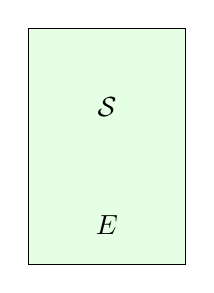
\begin{tikzpicture}
		\fill[green!10!white] (0,0) rectangle (2,3);
		\draw (0,0) rectangle (2,3);
		\node at (1,2) {$\mathcal{S}$};
		\node at (1,0.5) {$E$};
	\end{tikzpicture}
\end{center}

Sabemos então que vamos querer minimizar a entropia usual com

\begin{equation}
	U(S,V,N)  
\end{equation}

Com 

\[
	dU = TdS - PdV + \mu N
\]

e, especialmente

\[
\rho_E = \sum_{\sigma} \rho_\sigma = \Omega(E) \rho_\sigma
\]

Ou ainda, se $\Omega(E)$ é a quantidade de microestados,

\[
	 \rho_\sigma = \frac{1}{\Omega(E)}
\]

De forma que nossa função partição será

\[
	Z = \sum_\sigma \frac{1}{\Omega(E)} = 1
\]

E em relação a energia

\[
	Z = \sum_E \frac{1}{\Omega(E)} \Omega(E) = \exp{\left\lbrace \beta T k_b \log{\frac{1}{\Omega(E)}} \right\rbrace } \Omega(E) 
\]

Finalmente

\[
 \log{(Z)} = 0 = -\frac{S}{k_b} + \log(\Omega(E))
\]

Ou melhor

\begin{equation}
	S = k_b \log{(\Omega(E))}
\end{equation}